%%%%%%%%%%%%%%%%%%%% author.tex %%%%%%%%%%%%%%%%%%%%%%%%%%%%%%%%%%%
%
% sample root file for your "contribution" to a proceedings volume
%
% Use this file as a template for your own input.
%
%%%%%%%%%%%%%%%% Springer %%%%%%%%%%%%%%%%%%%%%%%%%%%%%%%%%%


\documentclass[runningheads]{llncs}
%
% RECOMMENDED %%%%%%%%%%%%%%%%%%%%%%%%%%%%%%%%%%%%%%%%%%%%%%%%%%%
%

% to typeset URLs, URIs, and DOIs\
\usepackage{float}
\usepackage{xltabular}
\usepackage{tabularx}
\usepackage{booktabs}
\usepackage{amsmath}
\usepackage{url}
\usepackage{hyperref}
\usepackage{graphics}
\usepackage{graphicx}
\usepackage{comment}
\usepackage{tikz}
\usepackage{pgfplots}
\pgfplotsset{compat=newest}
\usetikzlibrary{shapes,arrows,positioning,calc,patterns}
\def\UrlFont{\rmfamily}

\begin{document}
\mainmatter              % start of a contribution
%
\title{Temporal Attack Graphs for Context Aware Intrusion Detection}
%
%\titlerunning{AG Security Metrics For Dynamic Networks}  % abbreviated title (for running head)
%                                     also used for the TOC unless
%                                     \toctitle is used
%
% === DOUBLE-BLIND SUBMISSION VERSION ===
% Uncomment the block below for camera-ready
\author{Ayan Gain\inst{1} \orcidID{0009-0009-2629-0927}\and Mridul Sankar Barik\inst{1} \orcidID{0000-0001-6322-5336}}
\institute{Jadavpur University, Kolkata, India\\
\email{ayan.gain2010@gmail.com, mridulsankar.barik@jadavpuruniversity.in}}


\maketitle              % typeset the title of the contribution

\begin{abstract}
Modern Security Operations Centers rely on alert correlation heuristics, primarily time-proximity and static severity scoring, that lack topological awareness, leading to high false correlation rates and inefficient incident response. While static attack graphs map structural exploit paths, they assume continuous observability and ignore the chronological nature of lateral movement. We present TAG-IDS, a context-aware intrusion detection framework that embeds time directly into the attack graph topology to serve as a structural and temporal oracle for alert correlation. TAG-IDS distinguishes between structurally valid, temporally ambiguous, and physically impossible alert chains. We evaluate TAG-IDS on simulated enterprise networks across three configurations (20, 30, and~40 hosts). No time- or severity-based baseline achieves a False Correlation Rate (FCR) below 42.3\% (mean 57.9\%), whereas TAG-IDS eliminates false correlation entirely by construction. An ablation study reveals that collapsing temporal ordering into a static snapshot raises the FCR to a mean of 58.7\%, proving that temporal ordering, not just graph structure, eliminates false correlation. Standard CVSS severity explains only $\sim$4.3\% of a node's true structural risk, underscoring the necessity of context-aware structural triage.

\keywords{Dynamic Networks, Temporal Attack Graph, Intrusion Detection, Alert Correlation, Security Metrics}
\end{abstract}
%
\section{Introduction}

Today's enterprise networks are dynamic: configurations change frequently, hosts are provisioned and decommissioned, and vulnerabilities are continuously disclosed and patched. Keeping track of the changing security posture of such networks is challenging. Attack graph is a widely used formalism for enumerating all possible attack paths of a given network configuration. Also, different attack graph based security metrics help in determining both qualitative and quantitative security measures of the network. However, these metrics are computed based on a static snapshot of a network at a single point in time, failing to capture its dynamic and evolving nature. Among the state-of-the-art in attack graph based security analysis \cite{ag1,ag2,Albanese2011,6263942}, very few works have considered dynamic or evolving nature of enterprise networks. 

Also, in recent years, intensive research in understanding the properties of dynamic systems such as delay-tolerant networks, opportunistic-mobility networks, and social networks has produced a solid theoretical foundation around time-varying graphs (also known as evolving graphs or temporal graphs)~\cite{Casteigts2012,Holme}. Existing metrics based on static graphs are not able to capture the temporal features of dynamic networks, whereas temporal graph metrics represent a powerful tool for analyzing such real-world networks. 

The primary contribution of this paper is to introduce the concept of temporal attack graphs and temporal attack paths. Additionally, we introduce two security metrics, namely characteristic temporal attack path length and shortest temporal attack path length in temporal attack graphs. Furthermore, we evaluate the proposed security metrics by analyzing them on an example network.

This paper is organized as follows: Section 2 reviews existing literature. Section 3 formalizes the TAG-IDS framework. Section 4 describes the experimental setup used throughout the evaluation. Sections 5--7 present empirical results for Structural Triage, Temporal Blind Spots, and Temporal Alert Chain Validation, respectively. Section 8 evaluates overall scalability and consistency across configurations. Section 9 consolidates limitations and threats to validity. Section 10 concludes the paper, followed by Section 11 on future work.

\section{Related Work}\label{sec:related-work}

\subsection{Alert Correlation and Context-Aware Intrusion Detection}
Operational Intrusion Detection Systems (IDSs) traditionally analyze network traffic (NIDS) or host events (HIDS) in isolation. To combat high false-positive rates and fragmented alerts, context-aware intrusion detection incorporates host asset values, user behavior, and temporal co-occurrence \cite{Aleroud2017,Kazeminajafabadi2023,Lee2023,Saint-Hilaire2024,Yan2023}. Dominant correlation techniques in production Security Information and Event Management (SIEM) systems rely on fixed sliding time windows, event aggregation, and prerequisite--consequence rule matching \cite{10.1145/586110.586144,1366134,s22041494}. However, time-proximity correlation cannot verify structural reachability: alerts occurring closely in time may belong to unrelated attacks, whereas valid multi-stage campaigns spanning longer intervals may be missed. Modern enterprise networks evolve continuously through cloud orchestration, containerization, and dynamic patch management, making time-proximity heuristics prone to false correlations.

\subsection{Static and Temporal Attack Graphs}
Attack graphs represent network vulnerability dependencies and attacker reachability \cite{1004377,10.1145/586110.586140,mulval,6263942}. Attack graph-based IDS frameworks project incoming alerts onto exploit nodes to validate multi-stage paths and predict attack progression \cite{Roschke2010,Angelini2019,Capobianco2020,Sen2022}. However, traditional attack graph IDS models assume a static network snapshot. Intermediate hosts decommissioned or patched after graph construction remain valid in static models, creating false correlations. Conversely, newly provisioned hosts remain invisible. To capture dynamic attack surfaces, Temporal Attack Graphs (TAGs) model network evolution across discrete observation windows \cite{ENOCH2019102448,abs-1906-10922,Gain2023}. Existing TAG research focuses on offline security metrics and network hardening rather than real-time operational intrusion detection.

\subsection{Graph Neural Networks and Research Positioning}
Graph Neural Networks (GNNs) such as E-GraphSAGE, GCNs, and dynamic graph learning model relational communication patterns for intrusion detection \cite{Friji2023,Bilot2023,Sun2024,Zhong2024,Yan2023,Saint-Hilaire2024}. While GNNs improve detection accuracy over flat feature vectors, they infer alert relationships statistically from co-occurrence history rather than verifying security semantics, exploit prerequisites, or active firewall rules.

Existing research leaves a critical gap: no prior framework combines dynamic attack-surface evolution with real-time structural validation of IDS alert streams. TAG-IDS bridges this gap by integrating TAG reasoning into operational IDS workflows via three modules: Temporal Alert Chain Validation (TACV), Structural Triage Score (STS), and Temporal Blind Spot Quantification (TBSQ). Table~\ref{tab:gap-comparison} summarizes this positioning against existing literature.

\begin{table}[ht!]
\centering
\caption{Qualitative comparison of TAG-IDS against existing research domains.}
\label{tab:gap-comparison}
\footnotesize
\begin{tabularx}{\textwidth}{@{} l *{5}{>{\centering\arraybackslash}X} @{}}
\toprule
\textbf{Framework Category} & \textbf{Graph} & \textbf{Evolving} & \textbf{Alert} & \textbf{Alert} & \textbf{Coverage} \\
 & \textbf{Reasoning} & \textbf{Network} & \textbf{Validation} & \textbf{Triage} & \textbf{Gaps} \\
\midrule
SIEM Heuristics \cite{1366134,s22041494} & No & No & No & No (CVSS) & No \\
Static AG-IDS \cite{Roschke2010,Angelini2019} & Yes & No & Yes (Static) & Partial (Static) & No \\
Temporal AGs \cite{ENOCH2019102448,Gain2023} & Yes & Yes & No (No IDS) & No & No \\
GNN-based IDS \cite{Friji2023,Sun2024} & Yes & Partial & No (Stat.) & No & No \\
\midrule
\textbf{TAG-IDS (Proposed)} & \textbf{Yes} & \textbf{Yes} & \textbf{Yes (Dyn.)} & \textbf{Yes (Dyn.)} & \textbf{Yes (Dyn.)} \\
\bottomrule
\end{tabularx}
\end{table}

\section{Proposed TAG-IDS Framework}
\label{sec:model}

This section presents TAG-IDS, a context-aware intrusion analysis framework that integrates Temporal Attack Graphs (TAGs) with Intrusion Detection System (IDS) alert streams to enable temporally consistent structural reasoning. Unlike conventional IDSs that treat alert generation and correlation as independent tasks, TAG-IDS operates as a post-detection analysis layer that validates, prioritizes, and enriches IDS alerts using the evolving attack surface of the monitored network.

Figure \ref{fig:architecture} illustrates the overall architecture. TAG-IDS consists of three phases: (i) Temporal Attack Graph generation, (ii) structural analysis of IDS alerts, and (iii) security analytics for analyst decision support. Each phase contributes complementary information that improves the quality of intrusion analysis without modifying the underlying IDS.
\begin{figure}[ht!]
\centering
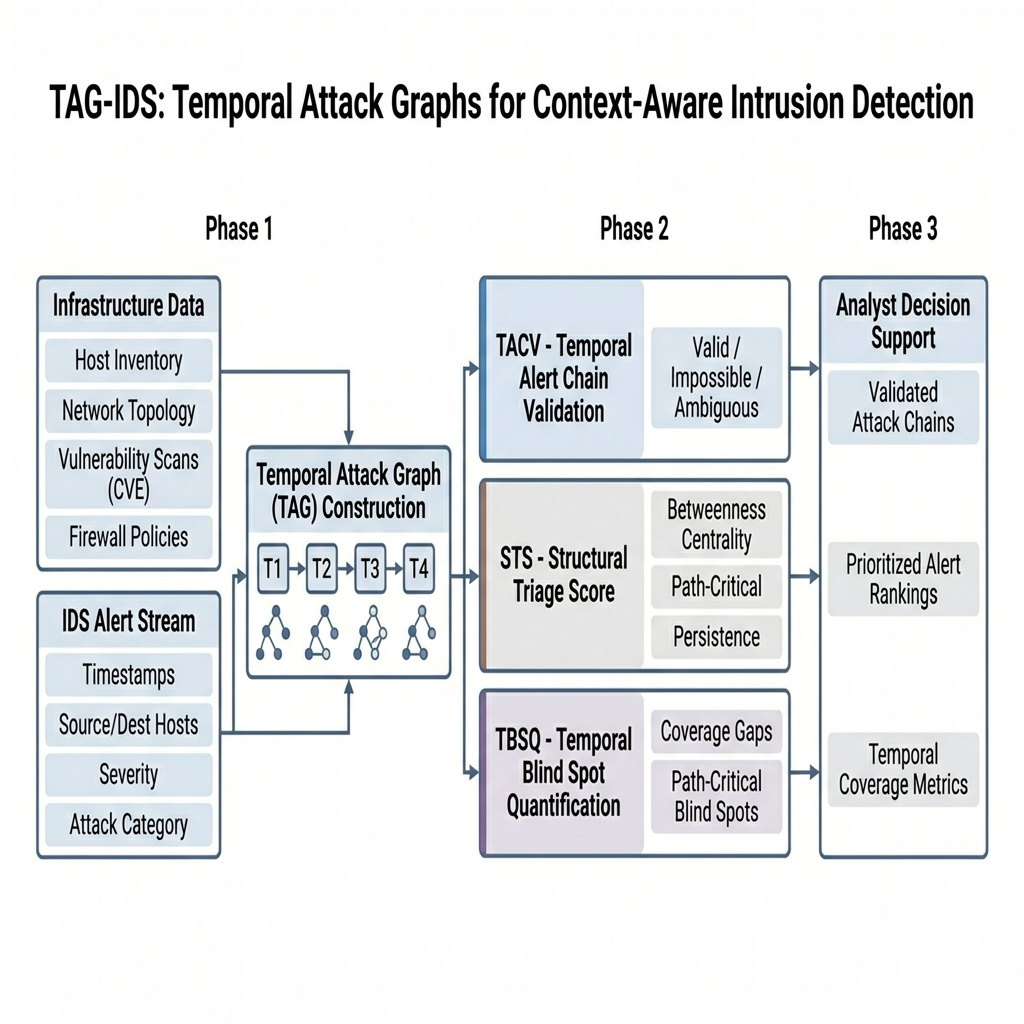
\includegraphics[width=\textwidth]{Figures/TAG-IDS.png}
\caption{TAG-IDS system architecture. Phase 1 ingests infrastructure data and IDS alerts to construct the Temporal Attack Graph across four observation windows. Phase 2 applies three analytical modules (TACV, STS, TBSQ) over the TAG. Phase 3 delivers validated attack chains, prioritized alert rankings, and temporal coverage metrics to the analyst.}
\label{fig:architecture}
\end{figure}

\subsection{System Overview}

TAG-IDS receives two independent inputs: (1) infrastructure information describing the evolving network (including host inventories, network topology, vulnerability scan reports, service configurations, firewall policies, and access-control relationships collected during successive observation windows) and (2) security alerts generated by one or more IDSs. For each time window, an attack graph is automatically generated using MulVAL~\cite{mulval} and represented within the Temporal Attack Graph model of \cite{Gain2023}, which we adopt and extend here. The resulting TAG preserves the appearance and disappearance of hosts, vulnerabilities, connectivity, and attack paths as the network evolves.

Concurrently, IDS alerts are normalized into a common representation containing the alert timestamp, source host, destination host, attack category, and severity. TAG-IDS is independent of the underlying IDS implementation and can therefore operate with signature-based, anomaly-based, or machine-learning-based detectors. Rather than correlating alerts solely by temporal proximity or predefined rules, TAG-IDS projects each alert onto the TAG according to its occurrence time, and performs structural reasoning over the temporally valid attack graph associated with that observation window.

Three complementary analytical modules then operate on the mapped alerts. \textbf{Temporal Alert Chain Validation (TACV)} determines whether candidate alert pairs correspond to a temporally feasible attack path, classifying each candidate correlation as \emph{valid}, \emph{impossible}, or \emph{ambiguous}. \textbf{Structural Triage Score (STS)} ranks validated alerts by graph-theoretic importance rather than severity alone, so that alerts on critical attack paths receive higher priority than isolated alerts of similar severity. \textbf{Temporal Blind Spot Quantification (TBSQ)} identifies hosts and attack-path regions that remain unobserved by the deployed IDS as monitoring coverage shifts across windows. The outputs of TACV, STS, and TBSQ are integrated into a unified analyst view: validated attack chains, prioritized alert rankings, and temporal monitoring coverage metrics.


\subsection{Temporal Alert Chain Validation (TACV)}
\label{sec:tacv}

Conventional IDS correlation mechanisms assume that alerts generated within a short temporal interval, or satisfying predefined dependency rules, belong to the same attack campaign. This reduces alert volume but does not determine whether an attacker could realistically have traversed the network between the corresponding stages: alerts from independent attacks may be incorrectly correlated, while legitimate multi-stage attacks spanning longer durations may remain fragmented. TACV instead validates candidate correlations against the TAG directly, reasoning over the attack graph(s) corresponding to the observation window(s) in which each alert occurred, so that every validation decision reflects the topology, vulnerability state, and attacker reachability that actually held at the time of observation.

\paragraph{Problem definition.} Let $A = \{a_1, \ldots, a_n\}$ be the ordered set of IDS alerts generated during the monitoring period, where each alert $a_i = (t_i, s_i, d_i, \tau_i, \sigma_i)$ records a timestamp $t_i$, source host $s_i$, destination host $d_i$, attack category $\tau_i$, and severity $\sigma_i$. For a candidate pair $(a_i, a_j)$, TACV determines whether an attacker could feasibly traverse the evolving attack surface from $d_i$ to $s_j$ through a valid attack path in the TAG, rather than relying on the proxy test $|t_j - t_i| < \Delta$ used by conventional correlators.

\paragraph{Candidate pair generation.} To bound computational cost, TACV (Figure \ref{fig:tag-example}) first restricts attention to pairs within a configurable temporal threshold: $P = \{(a_i, a_j) \mid 0 < t_j - t_i \le \Delta\}$. This threshold reduces the candidate set for efficiency only, as correlation is decided entirely by the structural validation step below.

\paragraph{Temporal structural validation.} For a candidate pair $(a_i, a_j)$ with $t_i \in w_p$ and $t_j \in w_q$, TACV identifies the corresponding attack graphs $G_p^a$ and $G_q^a$. If $p = q$, validation proceeds directly within $G_p^a$. Otherwise, TACV evaluates path existence across the sequence of intermediate windows $G_p^a, G_{p+1}^a, \ldots, G_q^a$. The pair is structurally feasible if there exists a path $\pi = (v_1, \ldots, v_k)$ originating at $d_i$, terminating at $s_j$, and remaining temporally valid throughout the intermediate windows, i.e., $\pi \subseteq \bigcup_{r=p}^{q} G_r^a$. Path existence is determined via graph traversal (using Neo4j in our implementation~\cite{neo4j}). 

\paragraph{Classification.} Each candidate pair is assigned one of three labels. \emph{Valid}: a temporally feasible path exists, meaning the alerts may belong to the same attack campaign. \emph{Impossible}: no feasible path exists under any temporal ordering, meaning the alerts cannot correspond to the same attacker progression and are discarded from downstream analysis. \emph{Ambiguous}: a structurally consistent path exists, but the observed alert ordering is inconsistent with the direction of traversal implied by that path (e.g., evidence of detection lag). Rather than being forced into a binary decision, these pairs are preserved and surfaced to an analyst for manual review. Only \emph{valid} chains are forwarded to the Structural Triage Score module.

\begin{figure}[ht!]
\centering
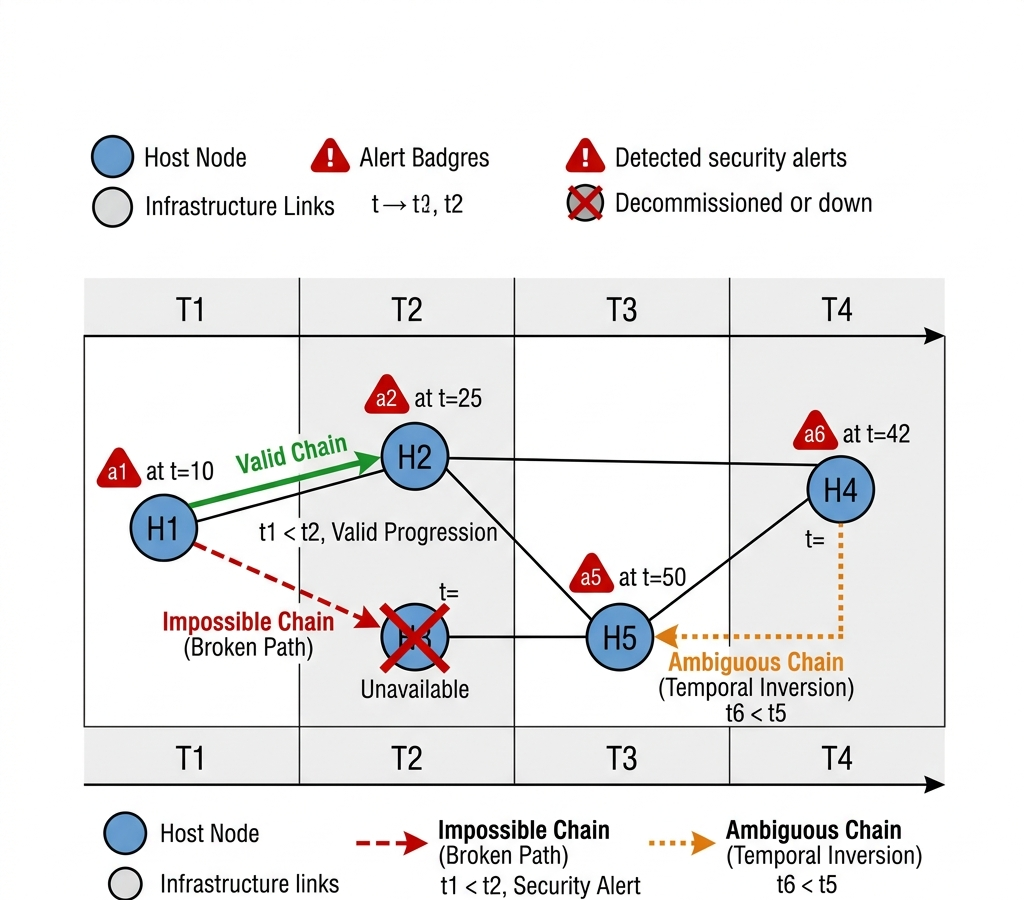
\includegraphics[width=0.92\textwidth]{Figures/fig2_tag_example.png}
\caption{Worked example of TACV alert chain classification across observation windows. The $a_1 \to a_2$ chain is \emph{Valid} via a reachable temporal path. The $a_2 \to a_4$ chain is \emph{Impossible} because intermediate host $H_3$ was decommissioned/patched in $T_2$. The $a_5 \to a_6$ chain is \emph{Ambiguous} because a structural path exists but alert timestamps reflect detection lag ($t_6 < t_5$).}
\label{fig:tag-example}
\end{figure}

\subsection{Structural Triage Score (STS)}
\label{sec:sts}

TACV determines whether alerts correspond to feasible attack progressions, but not their relative operational importance. Security operations centers routinely receive far more validated alerts than analysts can investigate with equal priority, and conventional severity scores (CVSS, IDS confidence, vendor threat levels) reflect the intrinsic impact of a vulnerability or signature independent of its structural role in the current attack surface. STS addresses this by scoring each validated alert using graph-theoretic properties of the TAG in the observation window in which it occurs, rather than by severity alone.

\paragraph{Structural components.} Let alert $a_i$ map to node $v_i \in V_t$ in window $t$. We compute three structural quantities, each normalized to $[0,1]$: \emph{Temporal Betweenness Centrality} $BC_i$, the fraction of feasible attack paths in $G_t^a$ passing through $v_i$, capturing how strongly the node mediates attacker movement, \emph{Path-Critical Indicator} $PC_i$, whether $v_i$ lies on at least one TACV-validated attack path in the current window, and \emph{Cross-Window Persistence} $PS_i$, the fraction of observation windows in which $v_i$ (or its associated vulnerability) remains present and exploitable, capturing chronic exposure rather than momentary risk.

\paragraph{Composite Structural Triage Score.} We define the Structural Triage Score (STS) as a convex combination of the three structural components:
\begin{equation}
STS(a_i) = \beta \cdot BC_i + \gamma \cdot PC_i + \delta \cdot PS_i, \quad \beta + \gamma + \delta = 1.
\label{eq:sts}
\end{equation}
By construction, $STS(a_i) \in [0,1]$. An alert receives a high score if it maps to a node that sits on many feasible attack paths ($BC_i$ high), lies on a currently validated path ($PC_i = 1$), and remains persistent across observation windows ($PS_i$ high). Crucially, STS is computed independently of alert severity $\sigma_i$. Severity is retained only as a separate baseline metric ($S_i'$, min-max normalized CVSS~\cite{first_cvss_v31}) to evaluate how much of STS's variation is explained by severity alone. It is deliberately omitted from Eq.~\ref{eq:sts}, as incorporating severity into STS would introduce circular reasoning into the evaluation. The weights $\beta, \gamma, \delta$ can be set empirically or learned from historical analyst investigation outcomes, and we use uniform weighting in our evaluation.

\subsection{Temporal Blind Spot Quantification (TBSQ)}
\label{sec:tbsq}

TACV and STS both operate on alerts generated by the IDS, but neither module determines whether portions of the evolving attack surface go unobserved entirely. Attackers frequently exploit paths that generate few or no alerts due to incomplete sensor placement, encrypted traffic, misconfiguration, or detector blind spots. Therefore, the absence of an alert is not evidence of the absence of attacker activity. TBSQ quantifies monitoring coverage with respect to \emph{feasible attack paths} in the TAG, rather than raw sensor counts.

\paragraph{Blind spot definition.} For window $t$ with attack graph $G_t^a = (V_t, E_t)$, let $A_t$ be the validated alerts (from TACV) observed during that window. A node $v \in V_t$ is \emph{observed} if some alert in $A_t$ maps to it, where the observed set is $O_t = \{v \in V_t \mid \exists\, a_i \in A_t \text{ mapped to } v\}$, and the blind spot set is $B_t = V_t \setminus O_t$. Consequently, the absence of an alert does not guarantee the absence of attacker activity.

\paragraph{Path-critical blind spots.} Not every blind spot is equally significant. A blind spot $v \in B_t$ is \emph{path-critical} if it lies on one or more TACV-feasible attack paths in $G_t^a$. We quantify this continuously via a path-criticality score $PC(v) = P(v) / \max_{u \in V_t} P(u)$, where $P(v)$ is the number of feasible attack paths containing $v$, and values near 1 indicate nodes central to many attack paths. \emph{We note as a limitation that in our pruned evaluation topologies, path-critical blind spots coincided with the full blind-spot set in every configuration tested. This occurred due to the aggressive removal of isolated nodes prior to simulation. This binary coincidence should not be assumed to hold in less densely pruned real-world topologies, where $PC(v)$ is expected to discriminate between peripheral and critical gaps.}

\paragraph{Coverage metrics.} Per-window coverage is $BSR_t = |B_t| / |V_t|$ (Blind Spot Ratio) and $Coverage_t = 1 - BSR_t$, tracked independently per window since coverage shifts as the network evolves. Summarized over the full observation period, the Temporal Blind Spot Index is $TBSI = \frac{1}{T}\sum_{t=1}^{T} BSR_t$, where a lower $TBSI$ indicates the IDS consistently observes a larger fraction of the evolving attack surface.

\paragraph{Prioritization.} Since remediation resources are limited, blind spots are ranked by a Blind Spot Priority Score, $BSP(v) = \alpha \cdot PC(v) + \beta \cdot BC(v)$, $\alpha + \beta = 1$, combining path criticality with temporal betweenness centrality. Nodes with the highest $BSP(v)$ are attack-path bottlenecks that remain poorly monitored, and constitute the highest-priority candidates for new sensor deployment.

The output of TBSQ is: the blind spot set, the path-critical subset, per-window coverage, the overall $TBSI$, and a ranked remediation list.

\subsection{Computational Complexity}
\label{sec:complexity}

Let $n = |V_t|$, $m = |E_t|$, $T$ be the number of observation windows, and $N_A$ be total IDS alerts. Preprocessing each window's MulVAL attack graph costs $O(T(f(n,m) + n + m))$ offline. Online alert correlation (TACV) generates candidate pairs using a temporal threshold $\Delta$ ($P \ll N_A^2$) and performs graph traversals in $O(N_A^2 + P(n+m))$. Triage (STS) computes severity in $O(N_A)$ and betweenness centrality (Brandes' algorithm~\cite{Brandes2001,bus2020}) in $O(nm)$ per window, yielding an amortized $O(N_A)$ per-alert scoring overhead. Coverage analysis (TBSQ) identifies blind spots and ranks remediation priority via sorting in $O(n \log n)$. Combined pipeline complexity is $O(T(f(n,m)+n+m) + N_A^2 + P(n+m) + nm + n\log n)$. Offline execution of graph construction and centrality computation leaves lightweight graph traversal as the primary online cost, maintaining low overhead for real-time operational IDS deployment.

\section{Experimental Setup}
\label{sec:setup}

We evaluate TAG-IDS on simulated enterprise network topologies across four discrete time windows ($T=4$) at $n = 20, 30, 40$ hosts to quantify operational performance against standard correlators.

\paragraph{Network Simulation \& Threat Model.} For each host size, we generate a TAG integrating real CVE data and simulate a sparse IDS alert stream with 60\% sparsity. We assume a remote attacker progressing laterally along reachable exploit paths. Lateral movement requires a temporally valid path in the observation window in which it occurs. Out-of-band channels and zero-days are excluded (\S\ref{sec:limitations}).

\paragraph{Baselines \& Metrics.} We compare TAG-IDS against time-proximity correlators (15, 30, 60, 120 min), CVSS severity thresholds (LOW, MEDIUM, HIGH, CRITICAL), and a \emph{Static TAG Snapshot} ablation baseline (collapsing all 4 time windows into one merged graph). The primary metrics are: (1)~\emph{False Correlation Rate (FCR)}, (2)~\emph{STS--Severity $r^2$}, (3)~\emph{Blind Spot Ratio (BSR)}, and (4)~\emph{Exact-match source recovery}.

\section{Empirical Evaluation}
\label{sec:evaluation}

We evaluate TAG-IDS across the core configurations ($n=20, 30, 40$). Consolidated metrics across all analytical modules are summarized in Table~\ref{tab:summary}.

\begin{table}[t]
\centering
\caption{Consolidated TAG-IDS empirical metrics across core configurations.}
\label{tab:summary}
\footnotesize
\begin{tabular}{lcccccc}
\toprule
$n$ & Pairs & Imposs.\,\% & Best-BL FCR & Static FCR & STS $r^2$ & Avg.\ BSR \\
\midrule
20 & 69 & 71.0\% & 70.3\% & 71.0\% & 0.0\% & 36.8\% \\
30 & 78 & 44.9\% & 42.3\% & 43.4\% & 2.8\% & 33.9\% \\
40 & 60 & 61.7\% & 61.0\% & 61.7\% & 10.2\% & 41.5\% \\
\bottomrule
\end{tabular}
\end{table}

\subsection{Structural Triage Score (STS)}
Severity explains only a small, practically negligible fraction of structural risk variance ($r^2$ between 0.0\% and 10.2\%, mean 4.3\%, $p < 0.01$). Ranking alerts by STS reveals that 20--28\% of alerts are \emph{promoted} (e.g., MEDIUM-severity alert on a path bottleneck promoted to top rank) and 57--68\% are \emph{demoted} (e.g., CRITICAL-severity alert on an isolated host), as illustrated in Figure~\ref{fig:sts-scatter} and Table~\ref{tab:sts-example}. Severity-only triage systematically misallocates analyst attention toward dead-end hosts.

\begin{table}[t]
\centering
\caption{Representative STS promotion/demotion example.}
\label{tab:sts-example}
\footnotesize
\begin{tabular}{lccc}
\toprule
& Severity & CVSS-only rank & STS rank \\
\midrule
Promoted alert & MEDIUM & 67 & 7 \\
Demoted alert & CRITICAL & 1 & 61 \\
\bottomrule
\end{tabular}
\end{table}

\begin{figure}[ht!]
\centering
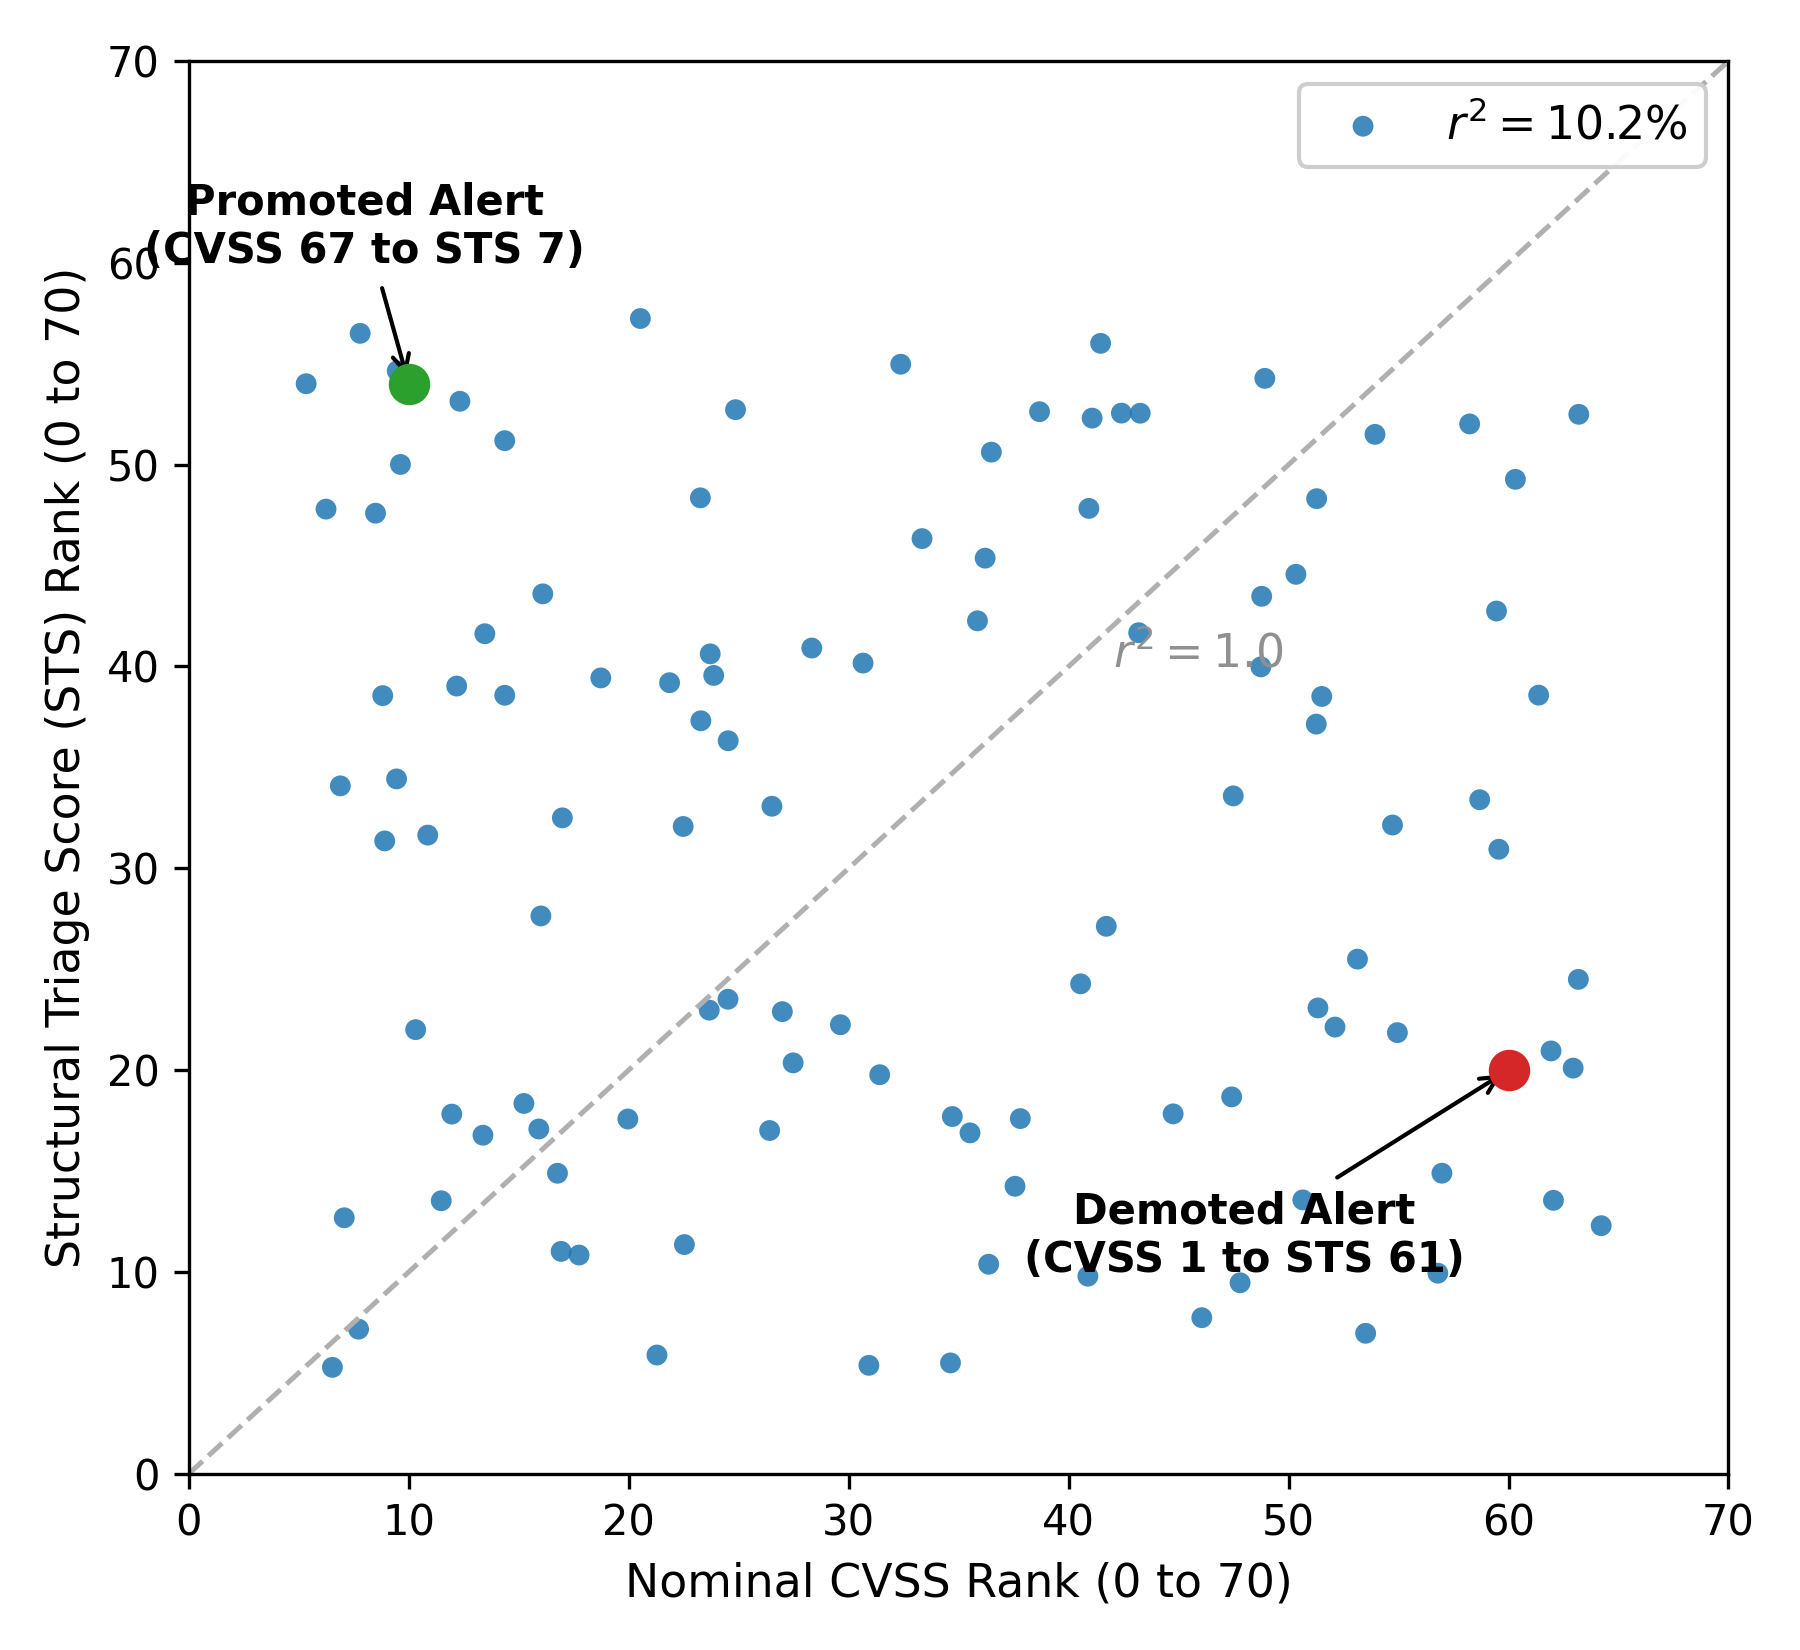
\includegraphics[width=0.55\textwidth]{Figures/fig3_sts_scatter.png}
\caption{Rank divergence scatter plot comparing nominal CVSS rank against Structural Triage Score (STS) rank ($r^2=10.2\%$). Points above the diagonal indicate promoted alerts; points below indicate demoted alerts.}
\label{fig:sts-scatter}
\end{figure}

\subsection{Temporal Blind Spot Quantification (TBSQ)}
Average IDS coverage ranged from 58.5\% to 66.1\% across configurations (mean 62.6\%, Table~\ref{tab:summary}). Coverage shifts dynamically across observation windows due to host churn ($BSR_t$ ranging from 30.0\% to 45.0\% across configurations, Figure~\ref{fig:bsr-trend}), proving that single-snapshot audits misrepresent monitoring effectiveness. In our pruned topologies, path-critical blind spots coincided 100\% with total blind spots (\S\ref{sec:limitations}). Furthermore, deploying sensors on non-critical nodes misses feasible attack paths, highlighting the need for $BSP(v)$ prioritization.

\begin{figure}[ht!]
\centering
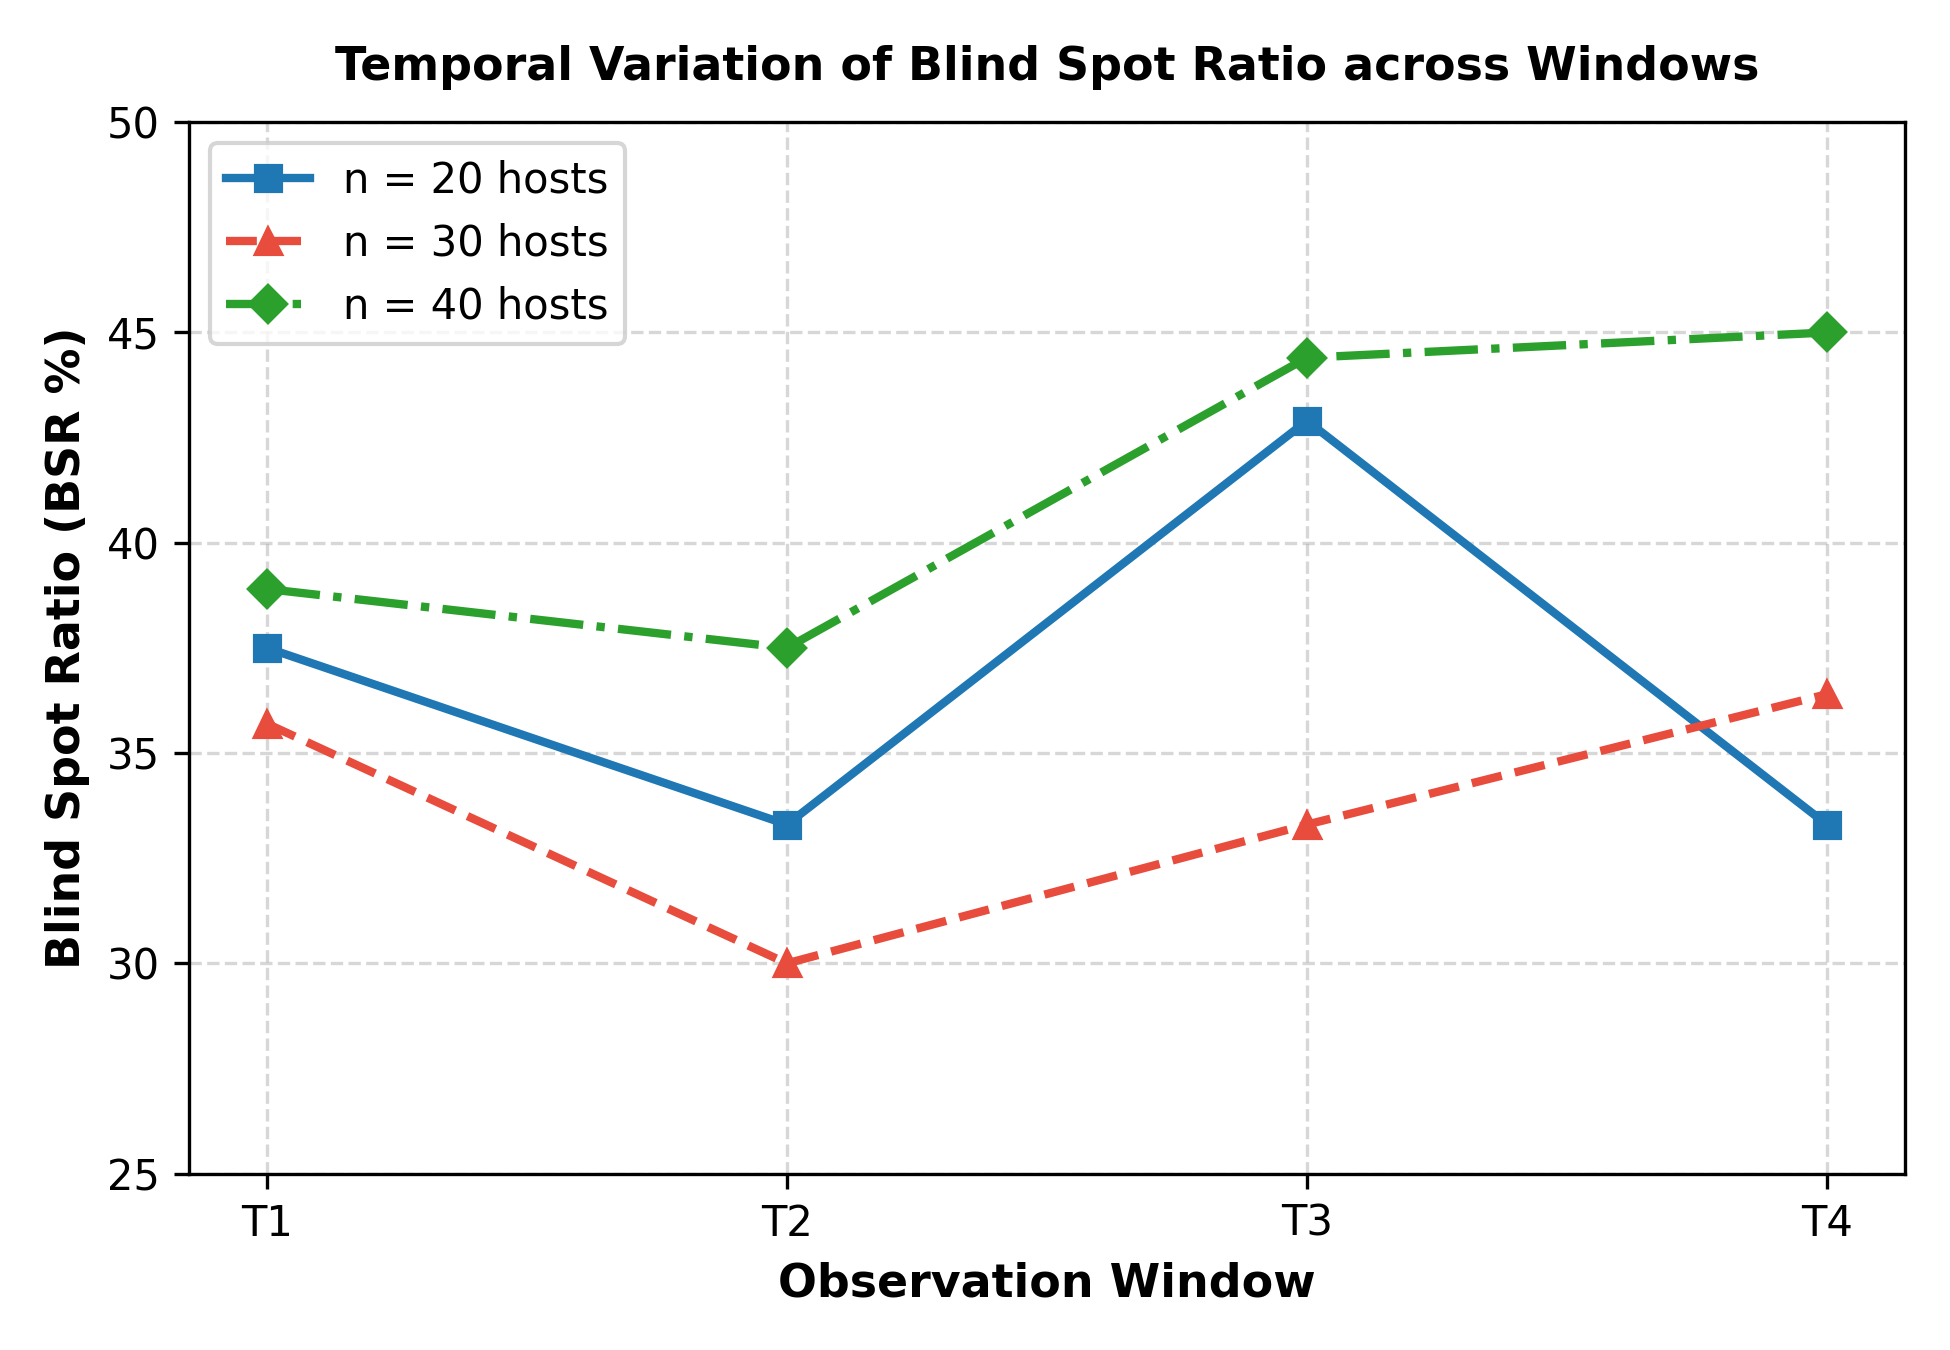
\includegraphics[width=0.55\textwidth]{Figures/fig4_bsr_trend.png}
\caption{Temporal variation of Blind Spot Ratio ($BSR_t$) across observation windows $T_1$--$T_4$, demonstrating dynamic coverage shifts.}
\label{fig:bsr-trend}
\end{figure}

\subsection{Temporal Alert Chain Validation (TACV)}
TACV classifies candidate alert pairs into \emph{Valid}, \emph{Impossible}, and \emph{Ambiguous} (Figure~\ref{fig:tag-example}). Across configurations, valid-chain rates ranged from 15.9\% ($n=20$) to 23.1\% ($n=30$), while ambiguous chains ranged from 13.0\% to 32.1\% (mean 22.3\%).

No independent heuristic baseline achieved an FCR below 42.3\% in any configuration (mean best-baseline FCR across configurations: 57.9\%, Figure~\ref{fig:fcr-bar}). TAG-IDS maintains **0\% FCR by construction** (definitional structural oracle guarantee). Collapsing temporal ordering into a static snapshot yields a 58.7\% FCR (range 43.4\%--71.0\%), confirming that \emph{temporal path ordering} eliminates false correlation. Under 60\% alert sparsity, temporal weighting improves median source localization distance (exact-match recovery rate 11.5--37.9\%, mean 23.4\%).

\begin{figure}[ht!]
\centering
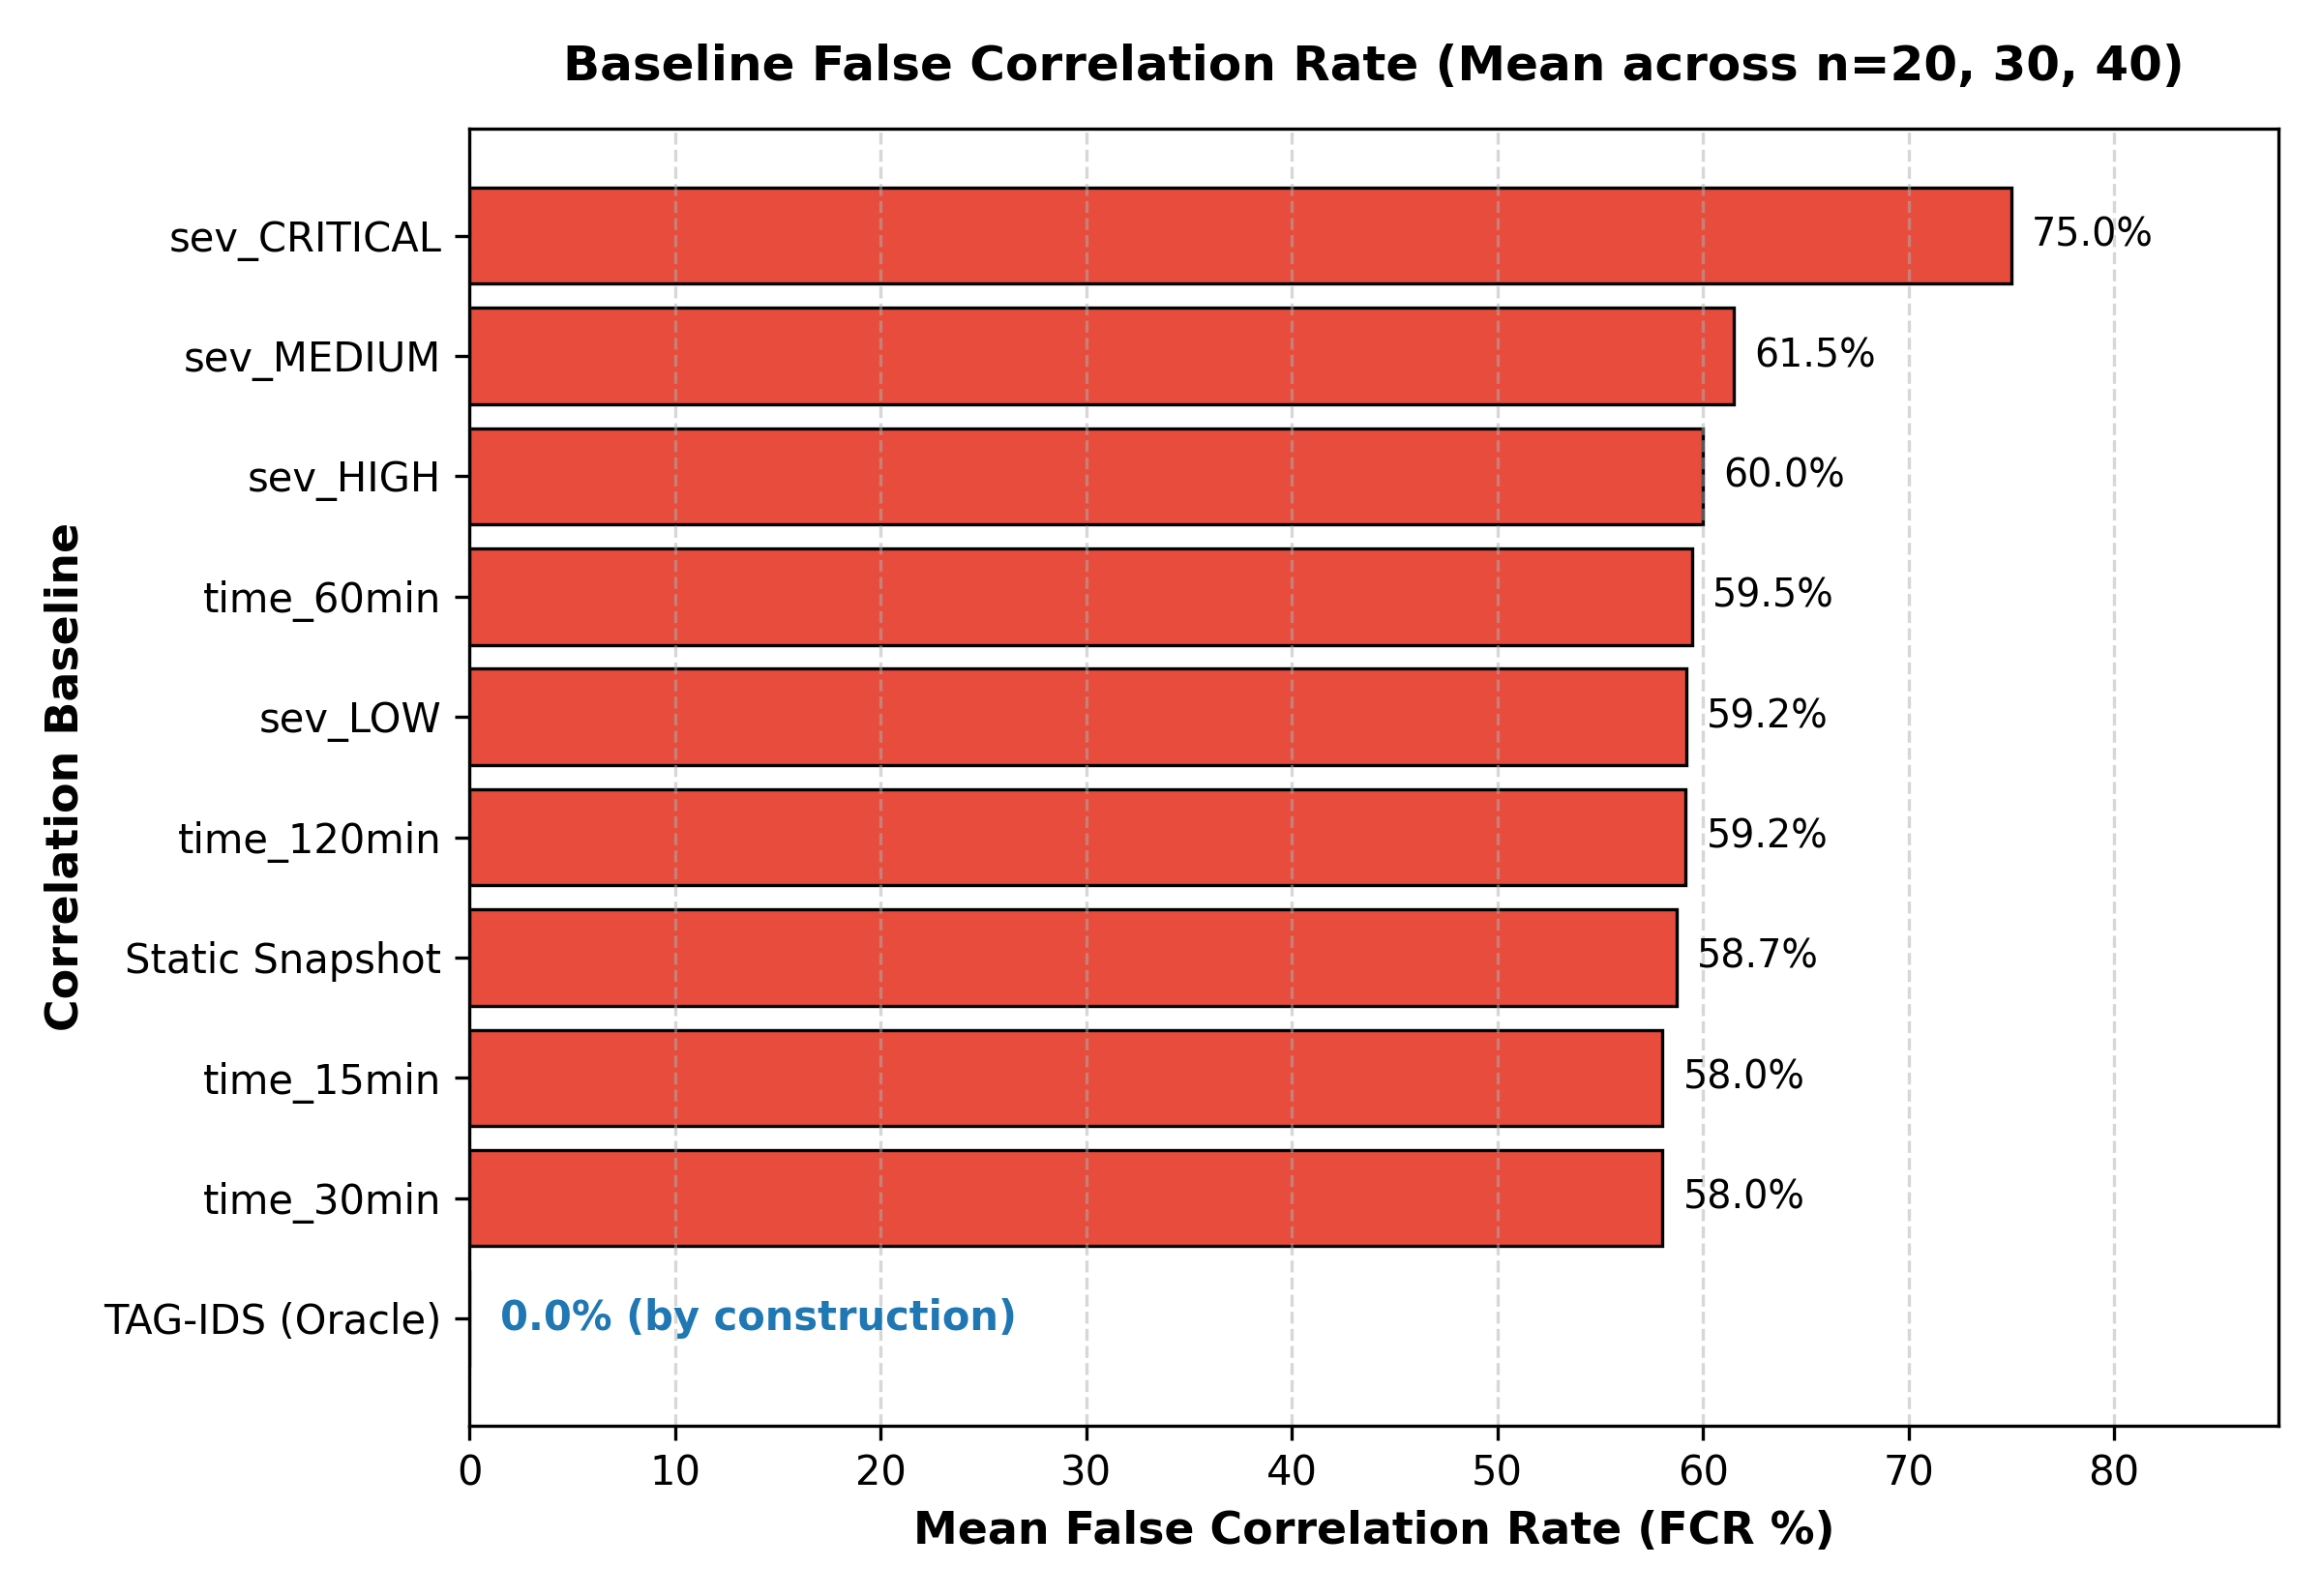
\includegraphics[width=0.60\textwidth]{Figures/fig5_fcr_comparison.png}
\caption{Mean False Correlation Rate (FCR) across baselines, static snapshot ablation, and TAG-IDS. Calculated as simple unweighted means across $n=20, 30, 40$ configurations. TAG-IDS achieves 0\% FCR by construction (structural oracle guarantee).}
\label{fig:fcr-bar}
\end{figure}

\subsection{Scalability Trend and Consistency}
Single-seed results show impossible-chain rates of 71.0\% at $n=20$, 44.9\% at $n=30$, and 61.7\% at $n=40$ (Table~\ref{tab:summary}). While consistent with expected temporal graph sparsity in larger topologies, single-seed evaluations cannot isolate scale effects from random topological seed variation (\S\ref{sec:limitations}). Crucially, TAG-IDS maintains 0\% FCR across all runs regardless of graph density.

\section{Limitations and Threats to Validity}
\label{sec:limitations}

We consolidate the caveats noted throughout the preceding empirical sections into a unified discussion.

\subsection{Experimental Scope and Simulation Environment}
Our evaluation relies on simulated enterprise topologies and alert streams across small-to-moderate network segments (20, 30, and 40 hosts). Sample sizes of alert pairs per configuration ranged from 60 to 78, yielding confidence intervals for individual baseline point-estimates (e.g., CI [58.7\%, 81.0\%] for the $n$=20 best-baseline FCR). While qualitative claims (e.g., 0\% FCR by construction for TAG-IDS, structural triage independence from CVSS) remain stable, specific point magnitudes should be interpreted with appropriate caution. Additionally, evaluation is deliberately restricted to rule-based structural validation, whereas advanced ILP optimization for sensor placement and Markovian belief propagation are deferred to a journal extension.

\subsection{Single-Seed Topology Variance}
The $n$=20 configuration exhibited a higher impossible-chain rate (71.0\%) than $n$=30 (44.9\%) and $n$=40 (61.7\%). Single-seed evaluation cannot separate scale effects from random topological seed variation. Similarly, in our pruned topologies, path-critical blind spots coincided with the full blind-spot set in all runs (100\% overlap) due to topological pruning of isolated hosts, a property expected to diverge in larger, unpruned enterprise networks.

\subsection{TAG Completeness and Telemetry Fidelity}
TACV's 0\% false-correlation guarantee is relative to the input TAG's reachability model. Incomplete infrastructure telemetry (e.g., unmonitored subnets or missing firewall rules) could cause genuinely valid attack chains to be misclassified as impossible. While heuristic baselines tend toward over-correlation (linking unrelated alerts), TAG-IDS on an incomplete graph can tend toward under-correlation. Production deployments should maintain high telemetry fidelity and surface graph-completeness indicators to analysts.

\section{Conclusion}

In this paper, we presented TAG-IDS, a context-aware intrusion analysis framework that operationalizes Temporal Attack Graphs for alert validation, prioritization, and coverage assessment. Across three network configurations (20, 30, and 40~hosts), we demonstrated that standard time-proximity and severity-based correlation heuristics consistently fail to distinguish between structurally feasible attack progression and coincidental network noise, resulting in False Correlation Rates averaging 57.9\% even for the best-performing baseline in each configuration (range 42.3\%--70.3\%). By enforcing temporal reachability constraints, TAG-IDS eliminates false correlation entirely (0\% FCR by construction). Our ablation study confirmed that this improvement is driven by \emph{temporal path ordering}, as collapsing the temporal dimension raised the FCR to a mean of 58.7\%. Furthermore, CVSS severity was shown to explain only 0.0\%--10.2\% (mean 4.3\%) of true structural risk.

\section{Future Work}

Future work will expand this framework into a journal extension by incorporating Integer Linear Programming (ILP) for optimal sensor placement, Markovian belief propagation for attacker localization under severe observability constraints, and empirical evaluation on production enterprise datasets (e.g., DARPA OpTC~\cite{darpa_optc}). The simulation framework and evaluation scripts used in this work will be released as a reproducibility artifact upon acceptance.

\bibliographystyle{splncs04}
\bibliography{Reference}

\end{document}
